% Eisenstein's lattice-point proof of reciprocity for p=7, q=11. Generated by a short script.
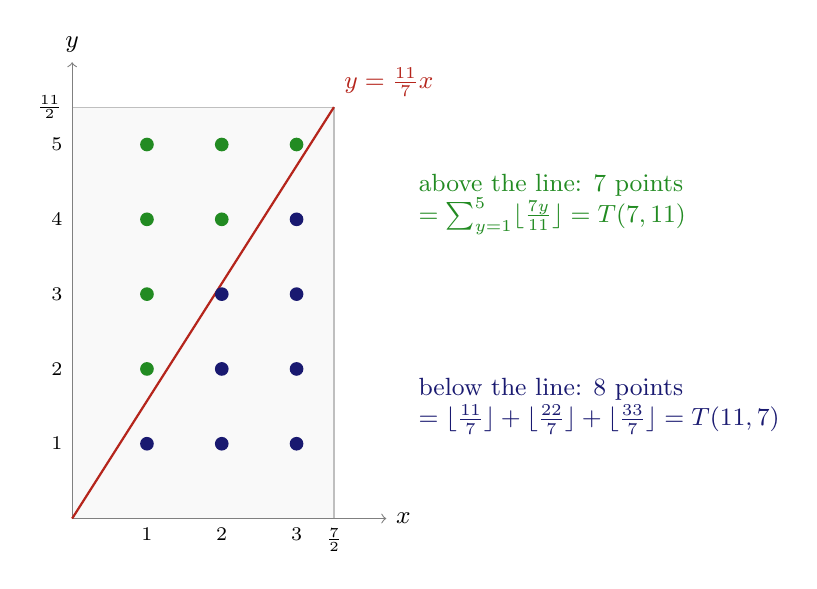
\begin{tikzpicture}[scale=0.95]
\draw[gray!50,fill=gray!5] (0,0) rectangle (3.5,5.5);
\draw[->,gray] (0,0)--(4.2,0) node[right,black,font=\small] {$x$};
\draw[->,gray] (0,0)--(0,6.1) node[above,black,font=\small] {$y$};
\draw[BrickRed,thick] (0,0)--(3.5,5.5) node[above right,font=\small] {$y=\frac{11}7x$};
\node[font=\scriptsize,below] at (3.5,0) {$\frac72$};
\node[font=\scriptsize,left] at (0,5.5) {$\frac{11}2$};
\node[font=\scriptsize,below] at (1,0) {1};
\node[font=\scriptsize,below] at (2,0) {2};
\node[font=\scriptsize,below] at (3,0) {3};
\node[font=\scriptsize,left] at (0,1) {1};
\node[font=\scriptsize,left] at (0,2) {2};
\node[font=\scriptsize,left] at (0,3) {3};
\node[font=\scriptsize,left] at (0,4) {4};
\node[font=\scriptsize,left] at (0,5) {5};
\fill[MidnightBlue] (1,1) circle (2.6pt);
\fill[ForestGreen] (1,2) circle (2.6pt);
\fill[ForestGreen] (1,3) circle (2.6pt);
\fill[ForestGreen] (1,4) circle (2.6pt);
\fill[ForestGreen] (1,5) circle (2.6pt);
\fill[MidnightBlue] (2,1) circle (2.6pt);
\fill[MidnightBlue] (2,2) circle (2.6pt);
\fill[MidnightBlue] (2,3) circle (2.6pt);
\fill[ForestGreen] (2,4) circle (2.6pt);
\fill[ForestGreen] (2,5) circle (2.6pt);
\fill[MidnightBlue] (3,1) circle (2.6pt);
\fill[MidnightBlue] (3,2) circle (2.6pt);
\fill[MidnightBlue] (3,3) circle (2.6pt);
\fill[MidnightBlue] (3,4) circle (2.6pt);
\fill[ForestGreen] (3,5) circle (2.6pt);
\node[MidnightBlue,font=\small,align=left,anchor=west] at (4.5,1.5) {below the line: 8 points\\$=\lfloor\frac{11}7\rfloor+\lfloor\frac{22}7\rfloor+\lfloor\frac{33}7\rfloor=T(11,7)$};
\node[ForestGreen,font=\small,align=left,anchor=west] at (4.5,4.2) {above the line: 7 points\\$=\sum_{y=1}^{5}\lfloor\frac{7y}{11}\rfloor=T(7,11)$};
\end{tikzpicture}
